\chapter{SRD}

\section{Introducción}

Introducir acá brevemente qué es un diodo SRD, sus diferencias con diodos
"usuales" de juntura, sus aplicaciones, y los aspectos que analizaremos.

El diodo SRD pertenece a una familia de dispositivos de juntura denominada
junturas de almacenamiento de carga \cite{moll1962}. Estos dispositivos se
caracterizan por su característica de recuperación reversa.

\section{Proceso de recuperación reversa}

En la figura \ref{fig:diode_reverse_recovery} se observa el proceso de recuperación reversa de un diodo. El mismo
se encuentra polarizado en directa con una corriente $I_f$, y en el instante
$t_0$ se aplica una corriente negativa $I_r$. Durante un tiempo $t_s$,
denominado tiempo de almacenamiento (\textit{storage time} en inglés), el diodo
permanece en un estado de baja impedancia, conduciendo corriente. Luego de este
tiempo, durante $t_t$ se da el tiempo de transición (\textit{transition time} o
\textit{decay time} en inglés). Durante este tiempo, la impedancia de la juntura
transiciona de bajo a alto, interrumpiendo la conducción de corriente. El tiempo
total $t_s+t_t$ es denominado tiempo de recuperación $t_r$.

\begin{figure}[t]
  \centering
    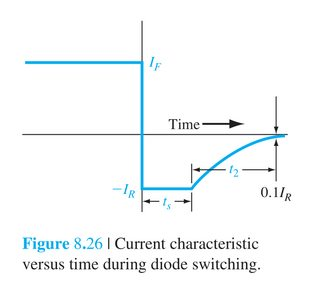
\includegraphics[width=0.4\textwidth]{images/diode_reverse_recovery.jpeg}
    \caption{Recuperación reversa de un diodo.}
    \label{fig:diode_reverse_recovery}
\end{figure}

Cada una de estas fases está relacionada a distintos procesos físicos que se dan
en la juntura. Cuando el diodo se encuentra en directa, la zona de vaciamiento
se reduce, resultando en un menor campo eléctrico, y una corriente neta de
difusión. Este mecanismo resulta en densidades de portadores minoritarios en los
extremos de la zona de vaciamiento proporcionales a $exp(V/V_t)$, resultando en
una inyección de portadores minoritarios en ambas partes de la juntura. Entonces
el diodo en directa tiene un exceso de portadores minoritarios.
\cite{neamen2012semiconductor}

El tiempo de almacenamiento $t_s$ está asociado al tiempo que demora la
corriente reversa $I_r$ en remover el exceso de portadores minoritarios de la
zona de vaciamiento. El tiempo de almacenamiento termina una vez que la densidad
de portadores minoritarios en los extremos de la zona de vaciamiento caen a sus
valores de equilibrio térmico.

Una vez terminado el tiempo de almacenamiento, las densidades de portadores
minoritarios en los extremos de la zona de vaciamiento cayeron a sus valores de
equilibrio térmico, pero en las zonas P y N todavía se encuentra una densidad de
portadores mayor a la de una juntura en reversa. El tiempo de transición $t_t$
esta asociado al tiempo que demoran estas densidades en caer a sus valores de
estado estacionario.

En la figura \ref{carrier_concentrations_turnoff} se observa la evolución
temporal de las densidades. Se observa que en $t=0^-$ las densidades en los
extremos de la zona de vaciamiento están en sus valores máximos, y en $t_4=t_s$
caen a sus valores de equilibrio térmico. Sin embargo, en este instante las
densidades en el cuerpo de la juntura no están en sus valores de estado
estacionario $t=\inf$.

\begin{figure}[t]
  \centering
    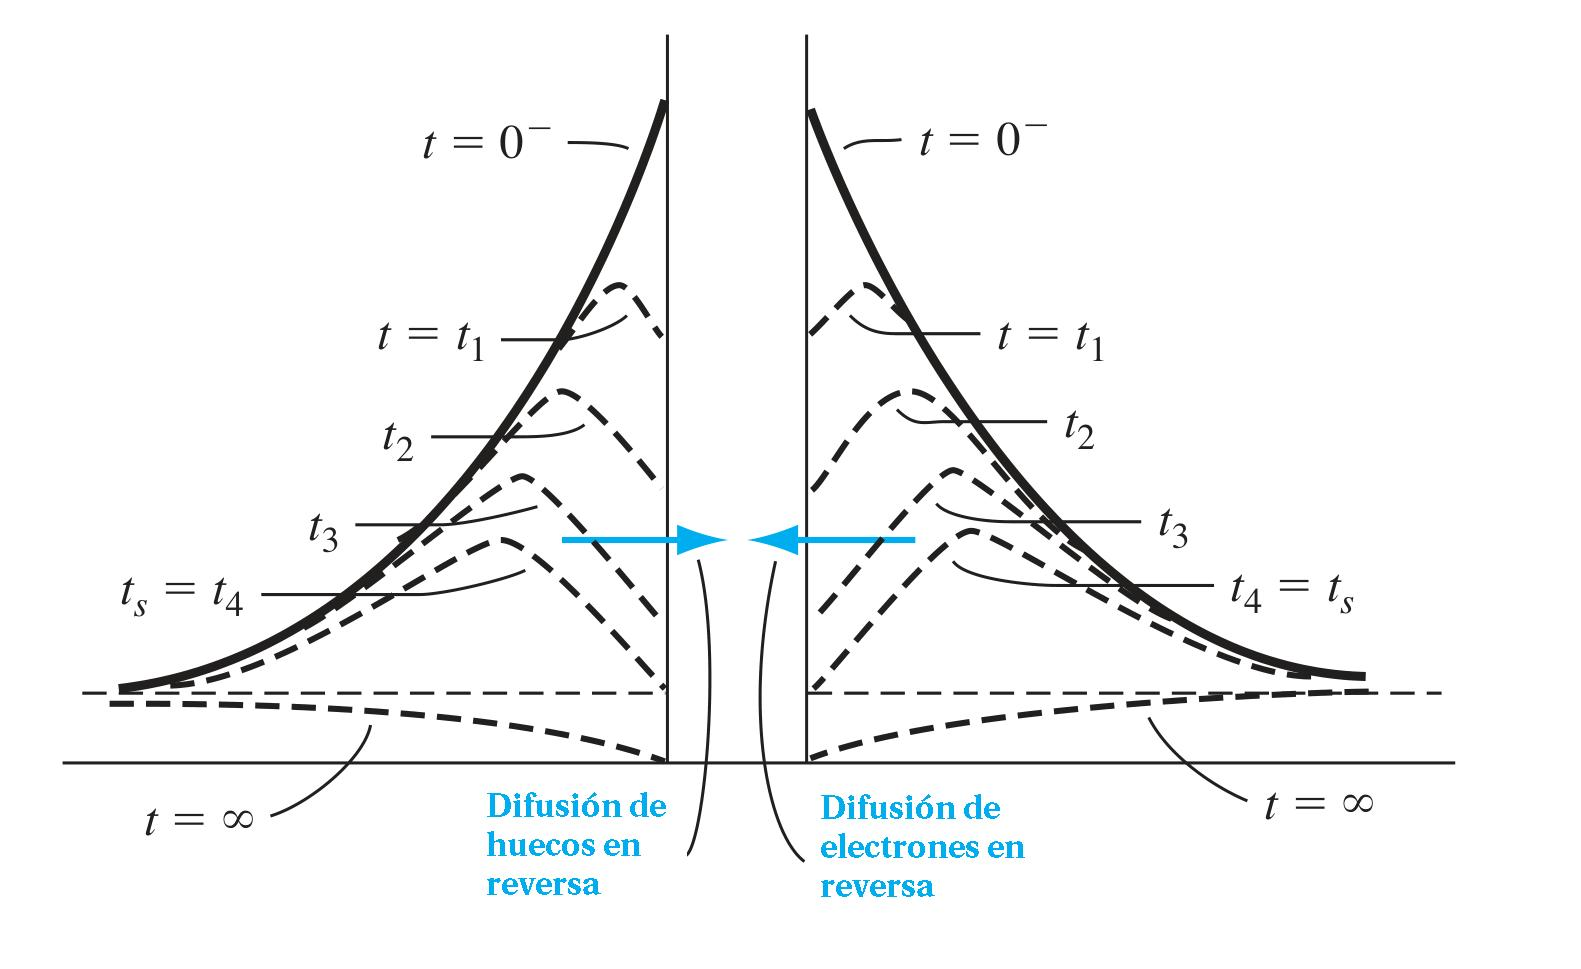
\includegraphics[width=0.4\textwidth]{images/carrier_concentrations_turnoff.jpg}
    \caption{Evolución de densidad de portadores en el proceso de recuperación.}
    \label{fig:carrier_concentrations_turnoff}
\end{figure}

\section{Diodos de almacenamiento de carga}
\label{sec:charge_storage_diodes}

En \cite{moll1962} de desarrolla la teoría de los diodos de almacenamiento de
carga. Estos se caracterizan por su particular comportamiento de recuperación
reversa.

En un diodo de juntura "usual", tanto el tiempo de almacenamiento como el de
transición tienen un orden de magnitud similar al tiempo de vida de los
portadores minoritarios $\tau_m$, o MCL del inglés \textit{Minority Carrier
Lifetime}. La característica distintiva de los diodos de almacenamiento de
carga, es que el tiempo de almacenamiento mantiene su orden de magnitud de
$\tau_m$, pero el tiempo de transición $t_t$ es mucho menor. \cite{moll1962}

En aplicaciones de conmutación de señal, es deseado que el tiempo de
recuperación $t_r$ sea lo menor posible. Esto minimiza las pérdidas de potencia
y maximiza la frecuencia de operación. En aplicaciones de generación de pulsos o
multiplicación de frecuencia, no es deseado un $t_r$ mínimo.

La combinación de tiempo de almacenamiento $t_s$ finito y tiempo de transición
$t_t$ muy corto es de utilidad en aplicaciones de generación de pulsos o
multiplicación de frecuencia. En la figura
\ref{fig:charge_storage_diode_waveforms} se observa el comportamiento de un
diodo de este tipo y uno con tiempo de recuperación 0.

En el caso del diodo llave ideal, la señal de salida sigue a la entrada cuando
esta es positiva, y es nula cuando la entrada es negativa, es decir, es un
rectificador ideal. En el caso de un diodo de almacenamiento de carga, hay un
tiempo de almacenamiento finito y comparable al período de la señal de entrada,
por lo que la señal de salida sigue a la entrada mientras esta es negativa.
Terminado el período de almacenamiento, el rápido tiempo de transición resulta
en un flanco de amplitud considerable y muy corto. Esta característica permite
generar pulsos ultra cortos o harmónicos altos de la señal de entrada.

\begin{figure}[t]
  \centering
    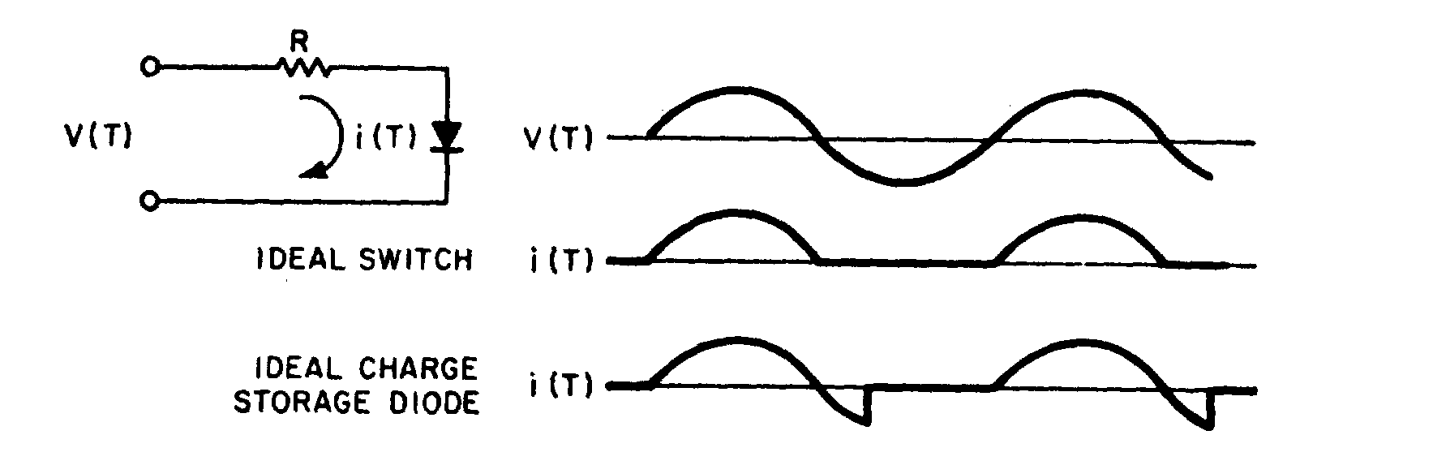
\includegraphics[width=0.4\textwidth]{images/charge_storage_diode_waveforms.jpg}
    \caption{Formas de onda en rectificadores}
    \label{fig:charge_storage_diode_waveforms}
\end{figure}

Los diodos de almacenamiento de carga implementan estas características de gran
tiempo de almacenamiento $t_s$ y tiempo de transición corto $t_t$. El tiempo de
almacenamiento prologando se obtiene implementando un MCL $\tau_m$ máximo
posible para el proceso de fabricación. El tiempo $t_t$ mínimo, se logra con un
diseño de diodo que resulte en una distribución de portadores en directa tal que
la mayoría de las cargas se encuentren muy cerca de la zona de vaciamiento. De
esta manera, una vez que las cargas de la zona de vaciamiento se remueven,
prácticamente no quedan cargas en el dispositivo, minimizando el tiempo de
transición $t_t$.

En \cite{moll1962} se demuestra que, siendo $x_0$ la distancia desde el centro
de la juntura al centro de gravedad de la distribución de portadores, el tiempo
$t_t$ será proporcional a $x_0^2/D$, con $D$ la constante de difusión promedio.

También se demuestra una relación inversa entre carga almacenada y velocidad de
transición $t_t$.

\section{Diodo SRD}
\label{sec:srd_diode}

El diodo SRD, del inglés \textit{Step Recovery Diode}, diodo de recuperación en
escalón, es un tipo de diodo de almacenamiento de carga, con las características
de los mismos descriptas anteriormente \cite{moll1969}.

El diodo es un un diodo PIN, es decir, un semiconductor intrínseco, la capa I,
entre dos semiconductores P y N. En la figura \ref{fig:srd_diode_structure} se
observa la estructura del mismo. La característica que diferencia al diodo SRD
de los diodos PIN usuales con aplicaciones en RF, es que en el SRD la capa I es
muy fina, entre \qty{0.5}{\micro\meter} y \qty{4}{\micro\meter}, mientras que en
un diodo PIN el rango es entre \qty{50}{\micro\meter} y
\qty{1000}{\micro\meter}.

El ancho de la capa I del diodo SRD le permite tener un MCL relativamente largo
y un tiempo de transición relativamente corto, características descriptas en
la sección \ref{sec:charge_storage_diodes} deseables para aplicaciones de generación de pulsos.

La capa I logra un dispositivo con un MCL considerable. Para lograr un tiempo de
transición lo más corto posible, como fuese explicado en la sección
\ref{sec:charge_storage_diodes}, es necesario que la mayoría de los portadores
minoritarios se encuentren alrededor de la zona de vaciamiento. Esto se logra
realizando un diodo $p^+in^+$, donde las zonas $p$ y $n$ están fuertemente
dopadas. Esto resulta en una almacenamiento de portadores en la zona intrinseca
$i$, y barreras de potencial que fuerzan a los portadores a mantenerse en la
zona $i$.

\begin{figure}[t]
  \centering
    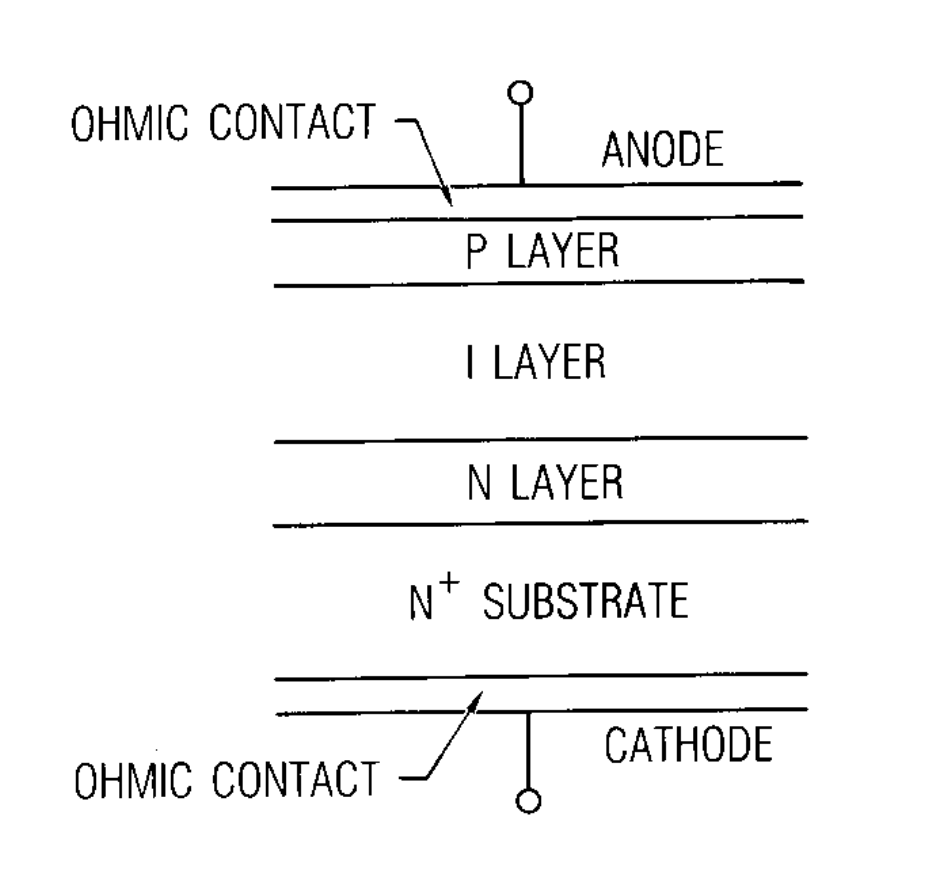
\includegraphics[width=0.4\textwidth]{images/srd_diode_structure.jpg}
    \caption{Estructura física del diodo SRD.}
    \label{fig:srd_diode_structure}
\end{figure}

\begin{figure}[t]
  \centering
    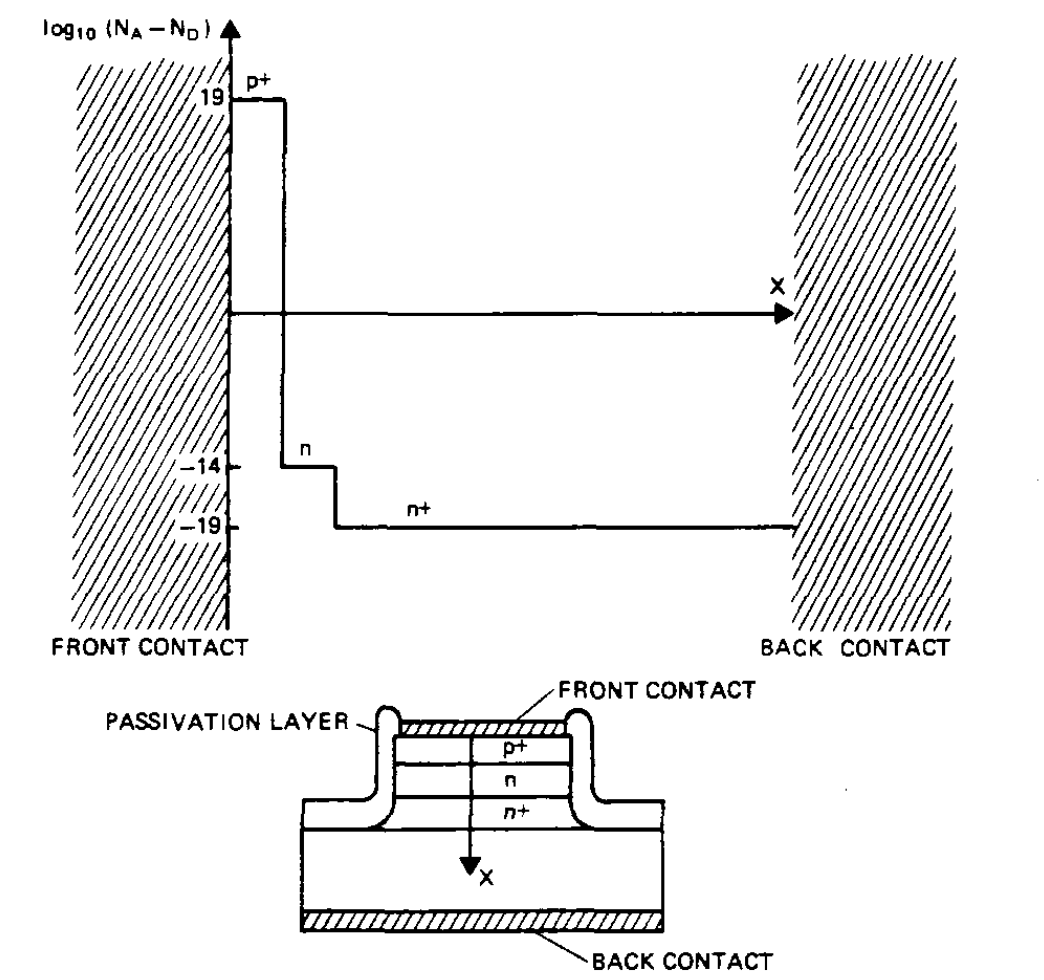
\includegraphics[width=0.4\textwidth]{images/srd_impurity_profile.jpg}
    \caption{Densidad de dopaje en SRD.}
    \label{fig:srd_impurity_profile}
\end{figure}

Para encontrar el tiempo de almacenamiento $t_s$ en un diodo SRD, puede
plantearse la ecuación de continuidad de carga \cite{moll1962} \cite{moll1969}

\begin{equation}
    \frac{dQ}{dt} = I-\frac{Q}{\tau_m}
\end{equation}

Esta ecuación contempla la inyección/remoción de carga mediante la corriente
externa $I$, y los efectos de recombinación de carga a través del tiempo de vida
de los portadores minoritarios $\tau_m$. En el caso de la corriente directa
$I_f$, puede plantearse la ecuación bajo $I=I_f$ y la condición inicial $Q(0)=0$para llegar a la carga almacenada $Q(t)$

\begin{equation}
    Q(t) = I_f \cdot \tau_m \cdot \left( 1-e^{-t/\tau_m}\right)
\end{equation}

Si se aplica la corriente $I_f$ durante un tiempo $T_f$, llegaremos a una carga
almacenada de

\begin{equation}
    Q_0 = Q(T_f) = I_f \cdot \tau_m \cdot \left( 1-e^{-T_f/\tau_m}\right)
\end{equation}

Para tiempos $T_f >> \tau_m$, será

\begin{equation}
    Q_0 \approx I_f \cdot \tau_m
\end{equation}

Para encontrar el tiempo de almacenamiento $t_s$, planteamos una corriente
constante $I=I_r$ y una condición inicial de $Q(0)=Q_0$. Queremos encontrar
$t_s$ tal que $Q(t_s) = 0$. Llegamos a

\begin{equation}
    t_s = \tau_m \cdot \ln \left( 1+\frac{Q_0}{I_r \cdot \tau_m}\right)
\end{equation}

Para el caso de $I_f$ constante, llegamos a

\begin{equation}
    t_s = \tau_m \cdot \ln \left( 1+\frac{I_f}{I_r}\right)
\end{equation}

Esta ecuación es valida para cualquier tipo de diodo de juntura, no solamente
PIN o SRD. En el caso del diodo SRD, el tiempo $\tau_m$ es considerable, por lo
que el tiempo de descarga $t_s$ es largo, típicamente decenas de nanosegundos, y comparable con el período de la señal de entrada.

Para el tiempo de transición $t_t$, en \cite{moll1969} se establece una regla
empírica que determina que será proporcional al largo de la zona $i$, con una
relación de \qty{10}{\pico\second} por cada \qty{1}{\micro\meter} de longitud.

El tiempo de transición es entonces, una cantidad que queda totalmente
determinada por el diseño del diodo. Esta variable tiene una dependencia con
otras, como por ejemplo la capacidad de reversa $C$ y la tensión de ruptura
$V_{br}$. Esta última disminuye con el volumen de la zona $i$, por lo que hay
una relación de compromiso entre $t_t$ y $V_{br}$. Siendo que este último valor
determina la potencia máxima en operaciones de multiplicación de frecuencia,
existe una relación de compromiso entre máxima frecuencia de operación y máxima
potencia \cite{moll1969}.

\section{Modelos circuitales y de simulación}
\label{sec:srd_simulation_models}

A orden 0, el diodo SRD puede ser modelado como un capacitor de dos estados: con
una capacidad infinita cuando el diodo se encuentra en directa, y una capacidad
muy baja en reversa, con un tiempo de conmutación 0 entre estados. La capacidad
de directa se corresponde con la capacidad de difusión del diodo, y la de
reversa con la capacidad de juntura. Este es un modelo que representa las
características de primer orden del diodo aceptablemente \cite{moll1969}.

Se puede mejorar este modelo incorporando los efectos de recombinación a la
capacidad de directa. Como fuese explicado en la sección \ref{sec:srd_diode}, la
recombinación puede ser contemplada incorporando en la ecuación de continuidad
el término $Q/\tau_m$, lo que tiene el efecto de una capacidad.

En la figura \ref{fig:srd_model_characteristics} se observa el modelo de SRD
junto a un gráfico de su capacidad en función del tensión.

\begin{figure}
    \centering
    \begin{subfigure}[b]{0.45\textwidth}
        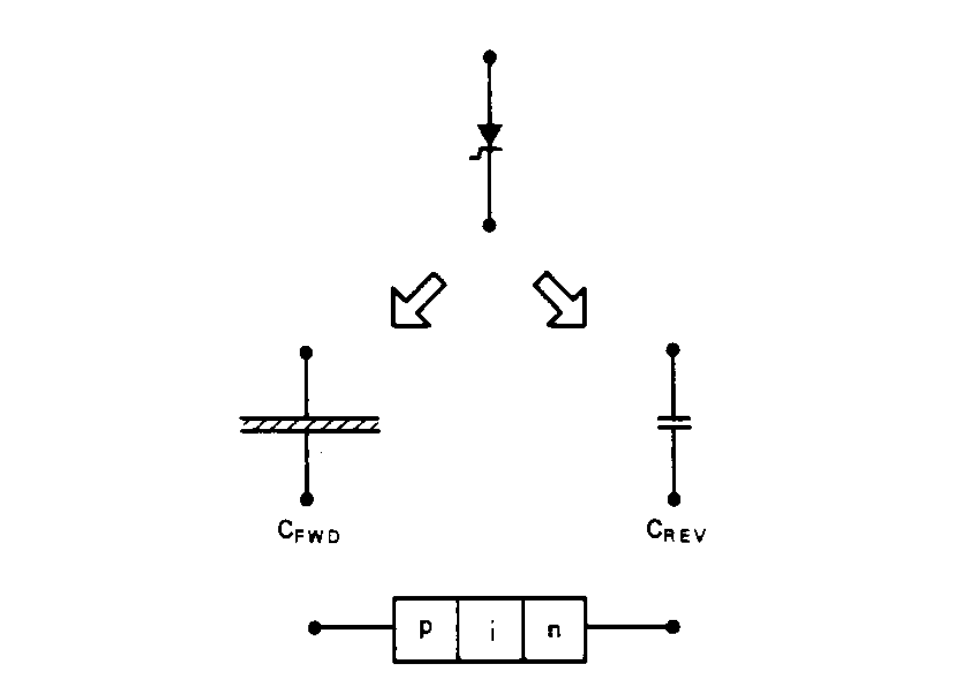
\includegraphics[width=\textwidth]{images/srd_switched_model.jpg}
        \caption{Modelo de capacidad conmutada del SRD.}
        \label{fig:srd_switched_model}
    \end{subfigure}
    \hfill
    \begin{subfigure}[b]{0.45\textwidth}
        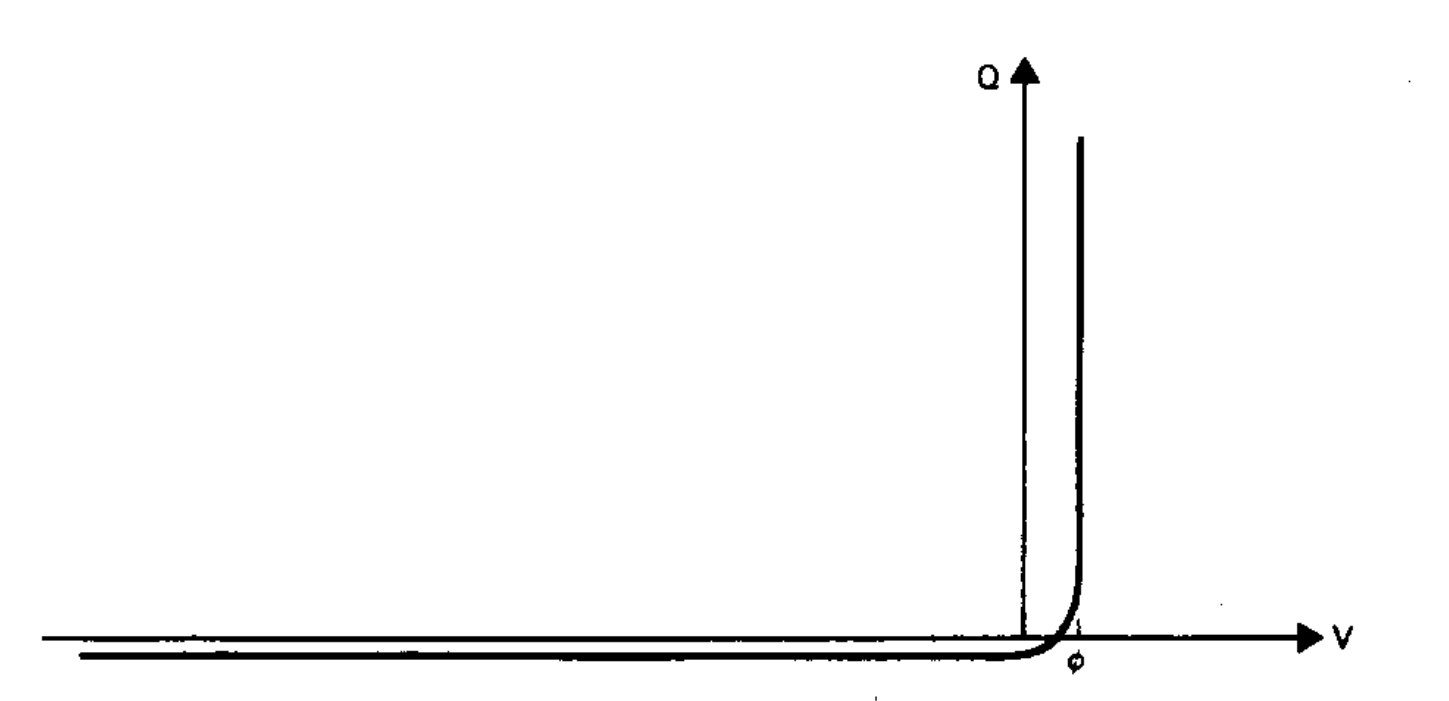
\includegraphics[width=\textwidth]{images/srd_capacity_vs_voltaje.jpg}
        \caption{Característica de capacidad en función de tensión para SRD.}
        \label{fig:srd_capacity_vs_voltaje}
    \end{subfigure}
    \caption{Características del modelo de SRD.}
    \label{fig:srd_model_characteristics}
\end{figure}

Para simular el diodo SRD, se utilizó un modelo de spice basado en este modelo
de capacidad de dos estados \cite{zhang1995} \cite{zhang1996}. Este modelo, que
puede observarse en la figura \ref{fig:srd_circuit_model}, está basado en un
modelo de capacidad conmutada en paralelo con una juntura PN.

Un problema del modelo de capacidad de la figura
\ref{fig:srd_capacity_vs_voltaje}, es la discontinuidad de la curva y su
derivada. Para mejorar este aspecto y tener un modelo utilizable en simuladores
comerciales, en \cite{zhang1995} se propone una mejora, Para modelar al
capacitor no lineal, se propone una relación entre carga y tensión lineal en 3
tramos, con valores que vuelven continua la curva y sus derivadas.

\begin{equation}
Q(V) =
    \left\{
    \begin{aligned}
        & C_r \cdot V  & V \leq 0 \\
        & c \cdot \left(V+a \right)^2 -b  & 0 < V < \phi \\
        & C_f \cdot \left( V - \phi \right) + Q_{rmp} & V \geq \phi \\
    \end{aligned}
    \right.
\end{equation}

En este modelo, la capacidad tiene un valor $C_r$ para valores de tensión
negativos, y $C_f$ para valores de tensión positivos. En el punto $V=\phi$, la
carga almacenada es $Q_{rmp}$, representando la carga residual en la juntura al
comienzo de la rampa de tensión descripta en la sección \ref{sec:srd_diode}.
Para la zona $0 < V < \phi$ se agregan constantes $a$, $b$ y $c$ para lograr una
curva continua. Se aplican las siguientes condiciones de contorno

\begin{equation}
    \left\{
    \begin{aligned}
        & Q(\phi) = Q_{rmp} \\
        & \frac{dQ}{dV}(\phi) = C_f \\
        & Q(0) = 0 \\
        & \frac{dQ}{dV}(0) = C_r \\
    \end{aligned}
    \right.
\end{equation}

Aplicando las condiciones de contorno, se llega a la siguiente relación

\begin{equation}
\label{eq:srd_non_linear_cap}
Q(V) =
    \left\{
    \begin{aligned}
        & C_r \cdot V  & V \leq 0 \\
        & \frac{C_f-C_r}{2\phi} \cdot \left(V+\frac{C_r\phi}{C_f-C_r} \right)^2
        -\frac{C_r^2}{2\left(C_f-C_r \right)}\cdot \phi  & 0 < V < \phi \\
        & C_f \cdot V - \frac{C_f-C_r}{2} \phi & V \geq \phi \\
    \end{aligned}
    \right.
\end{equation}

Para implementar esta capacidad no lineal, se necesitan los siguientes
parámetros:

\begin{itemize}
    \item $C_r$: esta es la capacidad de juntura del diodo, y es parte de las
        especificaciones del fabricante.
    \item $\phi$: es el potencial de juntura del diodo, especificado por el
        fabricante
    \item $C_f$: es la capacidad en directa del diodo. Se relaciona con el
        tiempo de vida de los portadores minoritarios $\tau_m$ y una resistencia
        dinámica $R_f$ a través de $\tau_m = C_f \cdot R_f$.
        \cite{Kotzebue1965}
\end{itemize}

La capacidad no lineal descripta en \ref{eq:srd_non_linear_cap} puede ser
implementada entonces con los datos provistos por el fabricante, solo siendo
necesario realizar una medición de la resistencia dinámica $R_f$. El modelo de
simulación final puede observarse en la figura \ref{fig:srd_circuit_model}.

En cuanto al alcance del modelo, este no contempla el tiempo de transición $t_t$
del diodo, por lo que sus efectos no están incluidos. Este modelo es suficiente
para análisis que involucren la carga y descarga del diodo, es decir, su
transición al estado de alta impedancia. El modelo no provee información sobre
la forma de esa transición.

Con esta curva se puede implementar el modelo de capacidad conmutada descripto
en \cite{moll1969} en una manera manejable para los simuladores de circuitos.
Bajo este modelo, se reportan en la literatura múltiples diseños de generadores
de pulsos \cite{Ruengwaree2006} \cite{Rahman2022} y multiplicadores de
frecuencia \cite{zhang1996} \cite{Heymann2001}, con buen acuerdo entre
simulación y medición.

Existen otros modelos de simulación para el diodo SRD, como los reportados en
\cite{Opalska1997} y \cite{Shevchenko2022} basados en balance de cargas. Sin
embargo, estos son más complejos en su implementación, ya que requieren
múltiples fuentes controladas y mediciones de diversos parámetros del diodo. Es
por esto que se utilizó el modelo de \cite{zhang1995}.

\begin{figure}[t]
  \centering
    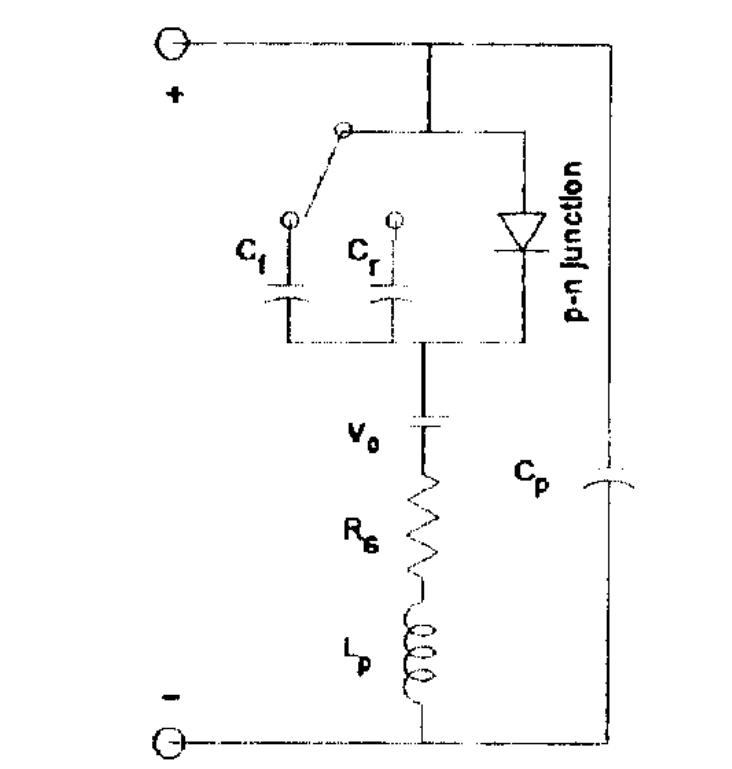
\includegraphics[width=0.4\textwidth]{images/srd_circuit_model.jpg}
    \caption{Modelo de simulación del SRD.}
    \label{fig:srd_circuit_model}
\end{figure}

\section{SRD utilizado}

Para la implementación del generador de pulsos de este trabajo, se seleccionó un
diodo SRD MMD830 de MACOM \cite{mmd830-datasheet}. Este pertenece a la familia
de diodos SRD MMDx.  Dentro de la familia, hay diversos modelos, con distintas
características. En la tabla se muestran algunos

Se decidió este diodo por un balance entre desempeño y costo. Al momento de su
adquisición, en agostod de 2022, el mismo tenía un costo de USD 54. Al momento
de la redacción de este trabajo, el costo del mismo es de USD 33. La gran
varación se debió al faltante de semiconductores que se experimentó en ese
momento. El dispositivo tiene un costo elevado a comparación de semiconductores
usuales que están en el rango de .1-5 USD, pero es un costo bajo como para
realizar una plataforma de bajo costo.

La familia viene en distintos tipos de encapsulados. Los hay desde bare die,
beam lead hasta plástico o cerámico. Dado los distintos parástios que cada
encapsulado tiene, tanto por su material como por su tamaño, el desmpeño de los
dispostivos presenta grandes variaciones. Por ejemplo, el tiempo de transición
$t_t$ más rápido de todos es de \qty{30}{\pico\second}, para el MMDB30-B11 en
en beam lead. Este presenta una capacidad de juntura de \qty{0.20}{\pico\second}
y una tensión de ruptura de \qty{14}{\volt}. En el otro extremo, el más lento de
todos es el MMD0803 en encapsulado de vidrio, con un tiempo de transición de
\qty{400}{\pico\second}, capacidad total de \qty{6.15}{\pico\farad}, y tensión
de ruptura de \qty{70}{\volt}

Entre los distintos encapsulados, se mantienen las figuras de tiempo de vida de
portadores $\tau_m$ y tiempo de transición $t_t$ para los mismos modelos. Lo que
cambia con el encapsulado, es la capacidad total $C_T$, incrementando con
mayores tamaños de encapsulado y resultando en una menor frecuencia de corte.

\begin{table}[t]
\centering
\begin{tabular}{|c|c|c|c|c|c|c|c|}
\hline
    \multirow{2}{*}{Modelo} & $V_B$ [V] &
    \multicolumn{2}{c|}{$C_j$ [pF]} & \multicolumn{2}{c|}{$\tau_m$ [ns]} &
    \multicolumn{2}{c|}{$t_t$ [ps]} \\
\cline{2-8}
    & Min & Min & Max & Min & Typ & Typ & Max \\
\hline
MMD805-0805-2 & 60 & 2.56 & 3.56 & 80 & 100 & 250 & 300 \\
MMD810-0805-2 & 50 & 1.75 & 2.75 & 40 & 70  & 200 & 250 \\
MMD820-0805-2 & 40 & 1.06 & 1.76 & 30 & 60  & 80  & 100 \\
MMD830-0805-2 & 25 & 0.56 & 1.06 & 15 & 30  & 60  & 80 \\
MMD832-0805-2 & 20 & 0.46 & 0.86 & 10 & 15  & 60  & 80 \\
MMD835-0805-2 & 15 & 0.36 & 0.86 & 10 & 20  & 50  & 70 \\
\hline
\end{tabular}
\caption{Desempeño de familia de SRD MMDx de MACOM.}
\end{table}

El encapsulado elegido es uno cerámico, el 0805-2. En la figura puede observarse
un diagrama del mismo, con sus dimensiones en mils y mm. Es un encapsulado muy
pequeño, de \qty{2.16}{\milli\meter}x \qty{1.40}{\milli\meter}. En la hoja de
datos se especifican su capacidad $C_p$ e inductancia $L_p$ parásitas en
\qty{0.06}{\pico\farad} y \qty{0.4}{\nano\henry} respectivamente.

\begin{figure}[t]
  \centering
    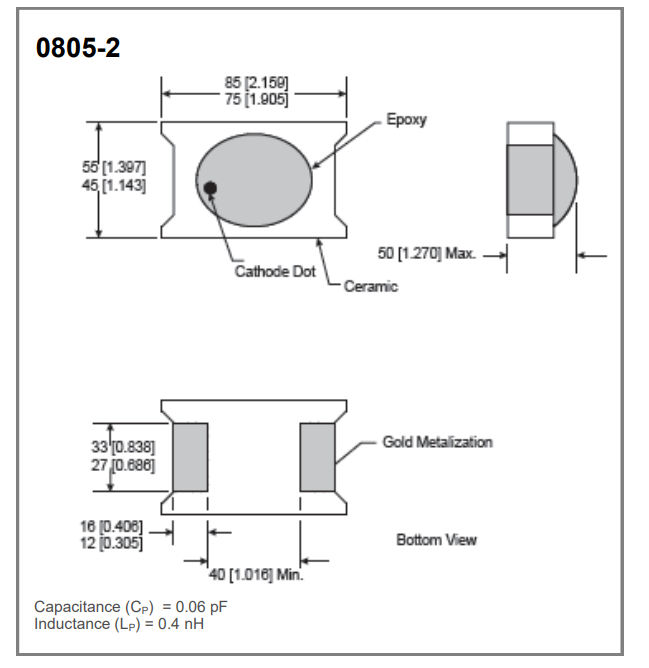
\includegraphics[width=0.4\textwidth]{images/srd_0805_outline.jpg}
    \caption{Dimensiones del encapsulado utilizado.}
    \label{fig:srd_0805_outline}
\end{figure}

\subsection{Validación de modelo}

Para validar el modelo propuesto para el SRD, y comprobar el desmpeño del diodo
seleccionado, se realizaron simulaciones en el software ADS.

En la figura \ref{fig:srd_model_ads} se observa el modelo implementado para el
SRD. El mismo contiene las inductancias y capacidad parásitas del encapsulado
$C_p$ y $L_p$.

\begin{figure}[t]
  \centering
    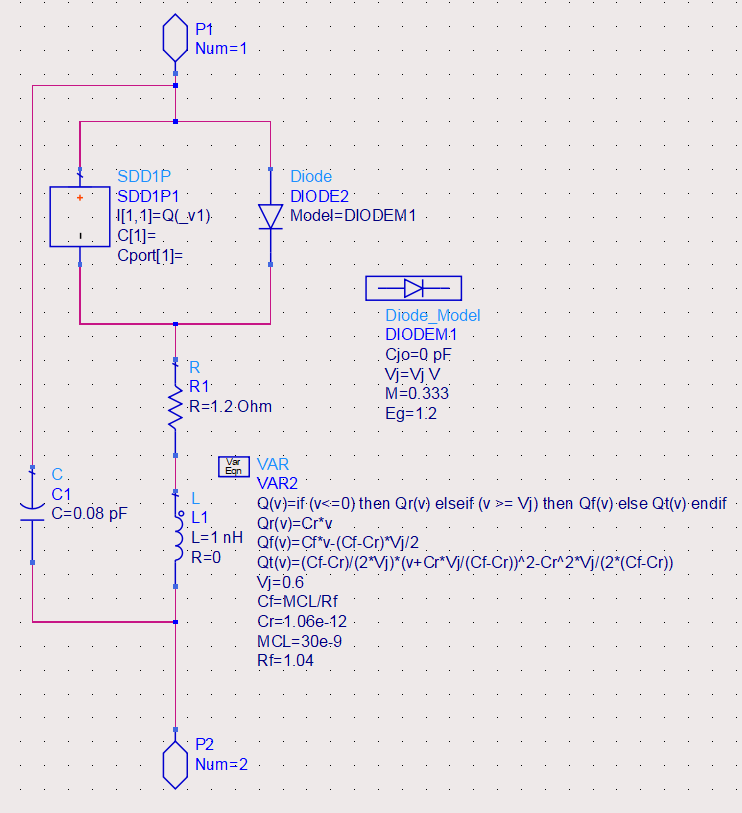
\includegraphics[width=0.4\textwidth]{images/srd_model_ads.jpg}
    \caption{Modelo implementado en ADS para el SRD.}
    \label{fig:srd_model_ads}
\end{figure}

Para modelar al diodo en sí, se colocan en paralelo una juntura PN y un
dispositivo definido simbólicamente. Este es un tipo de dispositivos disponibles
en ADS que permiten definir una relación arbitraria entre las variables del
dispositivo. En este caso, se define una relación entre la carga $Q(t)$ y la
tensión $v(t)$, definiendo de esta manera un capacitor no lineal. El capacitor
definido es el descripto en la sección \ref{sec:srd_simulation_models}.

Como el capacitor no lineal definido contempla tanto la capacidad de difusión
como la capacidad de juntura del diodo, en el modelo de diodo utilizado para
modelar la juntura, se define una capacidad de juntura de \qty{0}{\pico\farad},
para evitar modelar dos veces la misma. De esta manera, la juntura únicamente
modela la relación IV del diodo, $i_D(t) = I_S \left(
e^{\frac{v_D(t)}{V_T}}-1\right)$.

Con el modelo de SRD definido, se valida su comportamiento con una simulación.
En la figura \ref{fig:srd_validation_schematic} puede observarse el circuito
simulado. Consiste de una fuente de tensión en serie con el SRD y una
resistencia de limitación de corriente. Se simula el escenario dos veces con
estímulos distintos: una señal cuadrada y una senoidal, ambas de
\qty{10}{\mega\hertz} de frecuencia, \qty{10}{\volt} de amplitud pico-a-pico y
\qty{0}{\volt} de valor medio.

\begin{figure}[t]
  \centering
    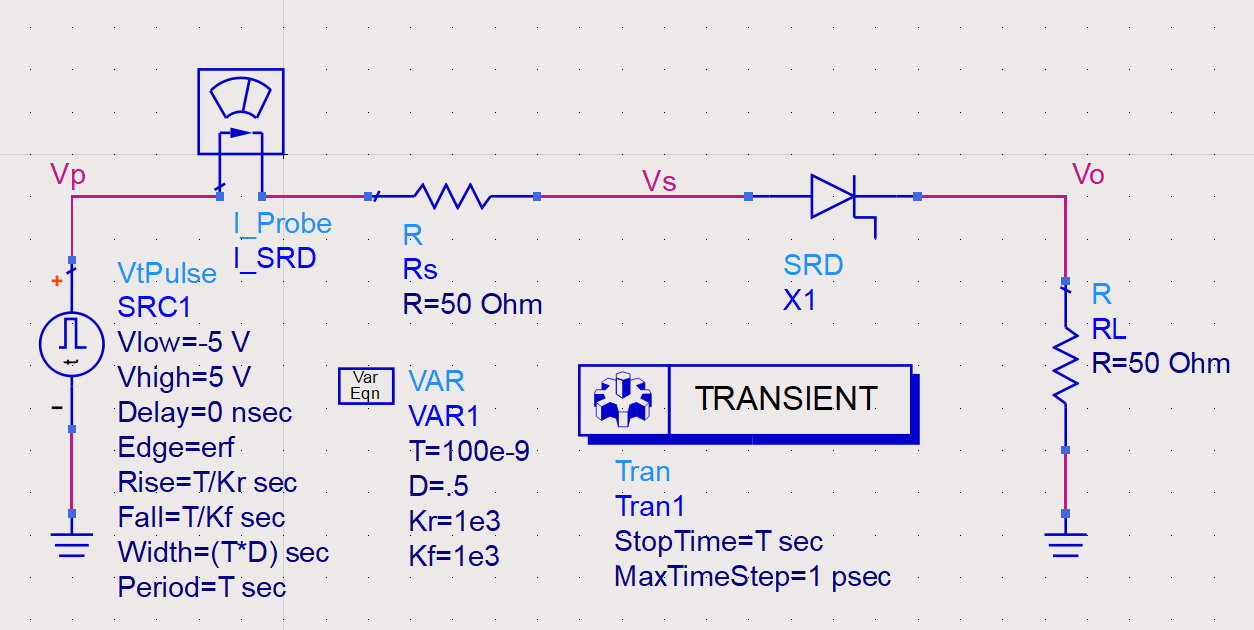
\includegraphics[width=0.4\textwidth]{images/srd_validation_schematic.jpg}
    \caption{Esquemático de simulación de modelo de SRD.}
    \label{fig:srd_validation_schematic}
\end{figure}

En la figura \ref{fig:srd_results} pueden observarse los resultados. En ambos
casos, para entrada senoidal y cuadarada, dado que no hay elementos resonantes,
corriente y tensión están en fase. En ambos ejes se observan las escalas. En
ambos casos, se observa como la salida sigue a la entrada, afectada por el
divisor de tensión de $R_L$ y $R_s$. Una vez que la corriente cambia el signo y
toda la carga del SRD es removida, este transiciona al estado de alta
impedancia, colapsando rápidamente la tensión a \qty{0}{\milli\ampere} y la
tensión de salida a \qty{0}{\volt}.

\begin{figure}
    \centering
    \begin{subfigure}[b]{0.45\textwidth}
        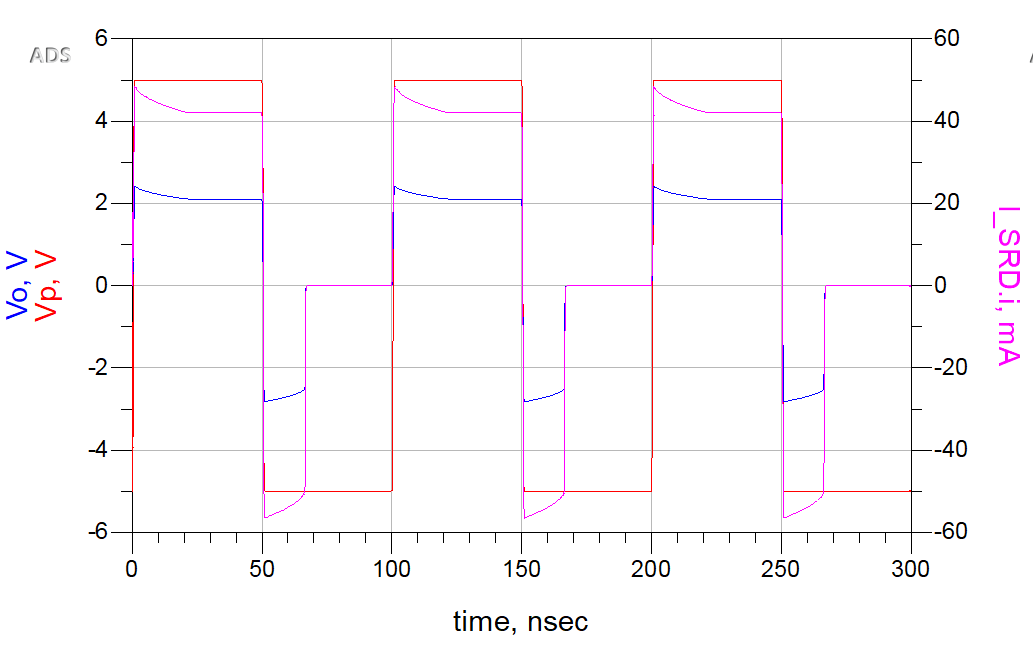
\includegraphics[width=\textwidth]{images/srd_result_square.png}
        \caption{Resultado de simulación con entrada cuadrada.}
        \label{fig:srd_result_square}
    \end{subfigure}
    \hfill
    \begin{subfigure}[b]{0.45\textwidth}
        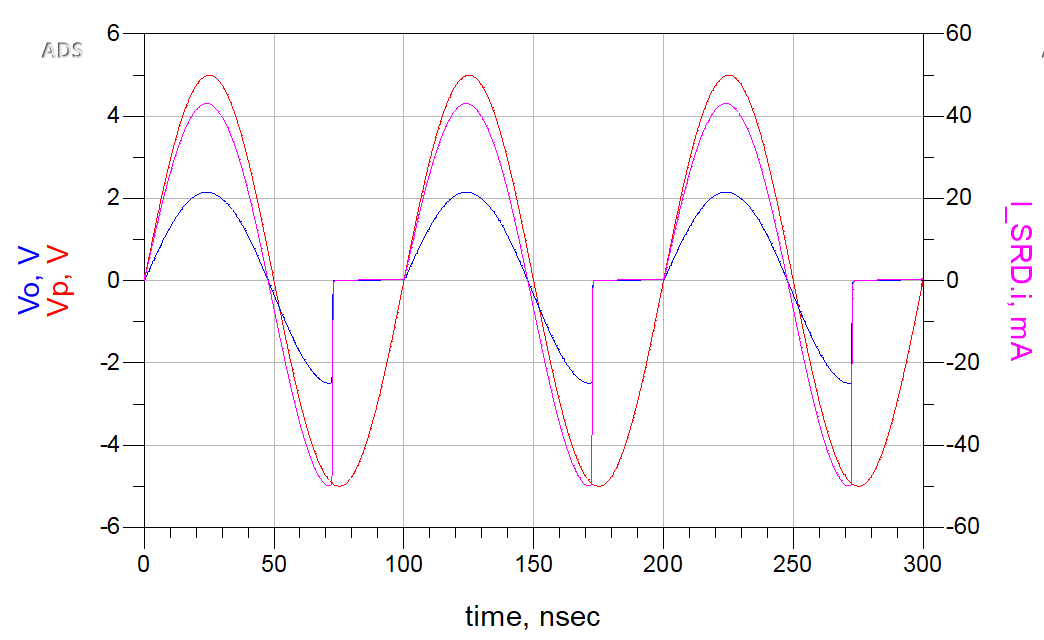
\includegraphics[width=\textwidth]{images/srd_result_sine.png}
        \caption{Resultado de simulación con entrada senoidal.}
        \label{fig:srd_result_sine}
    \end{subfigure}
    \caption{Resultados de simulación de modelo de SRD.}
    \label{fig:srd_results}
\end{figure}

Como fuese explicado en la sección \ref{sec:srd_simulation_models}, el modelo
utilizado contempla el tiempo de vida de los portadores minoritarios $\tau_m$,
pero no el tiempo de transición $t_t$. Por lo tanto, de estas simulaciones se
espera un correcto modelado del tiempo de almacenamiento $t_s$ pero no del
tiempo de crecimiento de la señal una vez terminado el tiempo de almacenamiento.

El tiempo de crecimiento de la señal dependerá tanto del tiempo de transición
del diodo $t_t$ como del circuito, a través de una constante de tiempo $t_{RC}$.
Si $R$ y $C$ son la resistencia y capacidad entre los terminales del SRD, el
tiempo de crecimiento $t_r$ será \cite{an918}

\begin{equation}
    t_r = \sqrt{t_t^2+t_{RC}^2}
\end{equation}

La capacidad $C$ estará compuesta por la capacidad de juntura del diodo y todas
las capacidades parásitas (de encapsulado y de PCB) que se encuentren. En la
simulación realizada, $t_t$ es nulo, por lo que el tiempo de crecimiento $t_r$
observado es igual a $t_{RC}$. En esta simulación la única capacidad es la de
juntura, en una simulación con extracción de parásitos, se contemplarían las
capacidades de las estructuras adyacentes.

*** *** *** *** *** *** *** *** *** *** *** *** *** *** *** *** *** *** *** ***
*** *** *** *** *** *** *** *** *** *** *** *** *** *** *** *** *** *** *** ***
*** *** *** *** *** *** *** *** *** *** *** *** *** *** *** *** *** *** *** ***
*** *** *** *** *** *** *** *** *** *** *** *** *** *** *** *** *** *** *** ***
*** *** *** *** *** *** *** *** *** *** *** *** *** *** *** *** *** *** *** ***
*** *** *** *** *** *** *** *** *** *** *** *** *** *** *** *** *** *** *** ***

\textcolor{red}{Hablar de dependencia de tiempo de crecimiento con carga
almacenada? Podemos decir que no tuvimos en cuenta esto por simplicidad.}

El diodo SRD es un diodo con un tiempo de vida de portadores minoritarios (MCL
del inglés \textit{Minority Carrier lifetime}). Esta característica resulta en
almacenamiento de carga en el mismo durante el período de conducción positiva.
De esta manera, si se aplica una corriente positiva y luego una negativa, el
dioodo permanecerá en un estado de baja impedancia, es decir, de conducción,
durante una porción de tiempo de corriente negativa. Es decir, la trancisión de
un estado de baja impedancia a uno de alta tiene un tiempo considerable.

Otra característica del diodo, es que una vez que la carga es removida, la
trancisión al estado de alta impedancia es muy rápida, del orden de los
picosegundos. Esta combinación de retraso en transición a estado de alta
impedancia y rápida conmutación, permite la generación de escalones de amplitud
de tiempo muy corto y amplitud considerable.

El retraso en la transición permite el desarrollo de una amplitud considerable
en el diodo. En comparación a un diodo usual, en el que transición es de muy
corto tiempo. Este retraso permite la generación de una amplitud considerable, y
luego se da un escalón de amplitud igual a esta, y con una velocidad igual a la
del diodo, que es muy rápido.

Al momento del apagado del diodo, su corriente cae a 0, resultando en una
tensión igual a 0 en su cátodo. En un diodo usual, con un bajo MCL, al momento
del apagado la tensión en el ánodo es pequeña en magnitud. En el caso de un
diodo SRD con un MCL considerable, en el momento del apagado la tensión del
ánodo se desarrolló hasta un valor considerable. La magnitud de está tensión
dependerá de la relación entre la constante de crecimiento de la fuente que
mueva al ánodo y el MCL. De esta manera, al momento del apagado se genera un
escalón de amplitud considerable. La velocidad de esta transición depende de la
velocidad de transición intrínseca del diodo y de los parásitos del nodo, y dada
la gran velocidad del diodo este escalón será rápido.

En cuanto a la geometría del diodo, este es un diodo PIN, es decir, un diodo con
una capa de semiconductor intrínseco entre dos capas P y N. Para el diodo SRD,
la capa I debe ser muy fina. Esto es mejor que un diodo con un dopaje lineal.

El tiempo de recuperación de un diodo SRD está limitado por el tiempo de
descarga de la capacidad de juntura.

A orden 0, el diodo SRD puede modelarse como un capacitor de dos estados: en
directa como un capacitor de capacidad infinita, y en reversa como un capacitor
de capacidad muy pequeña, con tiempo de transición 0 entre estados
\cite{moll1969}.

Un modelo más fidedigno, incorpora los efectos de recombinación para expresar a
$C_{fwd}$ como una capacidad finita, dada por el MCL.

En cuanto al tiempo de transición $t_t$, podemos mejorar el modelo y
considerarlo finito, y estará dado por el tiempo que demoran en extraerse los
portadores libres en el volumen de ancho $W$ y área $A$ (¿de la zona I?). En
esta transición, también habrá una perdida de potencia por conmutación.

El tiempo de transición $t_t$ está relacionado al ancho $W$ y el área $A$ de la
capa I. Por lo tanto, también a $V_{BR}$ y $C_{REV}$, y por lo tanto a la
capacidad de disipación de potencia, que es proporcional a $V_{BR} \cdot C_{REV}
\cdot f$. Por lo que tendremos una relación de compromiso entre tiempo de
transición y disipación de potencia. \textcolor{red}{Buscar de donde sale esa
relación con potencia disipada}

El modelo de capacidad conmuta tiene una histeresis. Cuando se conmuta desde el
estado de directa al de inversa, esta conmutación no es instantánea, ya que se
requiere la remoción de toda la carga almacenada. En el modelo ideal de
capacidad $C_{FWD}$ infinita, la carga a remover es toda la carga inyectada
durante el período de conducción. Cuando contemplamos el MCL, la carga contempla
la que ya fue recombinada, por lo que el tiempo se vuelve menor.

Para contemplar los efectos de recombinación, planteamos la ecuación de
continuidad teniendo en cuenta el MCL

\begin{equation}
    \frac{dQ}{dt} = I-\frac{Q}{\tau_R}
\end{equation}

Una corriente constante $I_F$ resultará en una carga almacenada de

\begin{equation}
    Q_F = I_F \cdot \tau_R
\end{equation}

El tiempo de descarga será el tiempo que le toma a la corriente negativa remover
toda esta carga almacenada $Q_F$.

Cuál es la diferencia entre MCL y transit time? En \cite{maas2003} dice que, por
separado, el SRD debe

\begin{itemize}
    \item Tener un tiempo largo de almacenamiento, i.e. tiempo largo de
        recombinación
    \item Tener una zona de vaciamiento angosta, para que los efectos de tiempo
        de transito no afecten la eficiencia en altas frecuencias
\end{itemize}

Entonces, no son lo mismo. Parecería que sí, en otras derivaciones donde se
obtienen expresiones para las transiciones de on-off en un PN usual, y el
transit time se usa casi igual que el MCL acá.

El tiempo largo de recombinación, permite que se inyecte carga en la región I y
que está NO se recombine, es decir, quede almacenada ahí. Si el tiempo de
recombinación fuera corto, la carga no se almacenaría, porque se vería
recombinada rápidamente.

En reversa, la región de vaciamiento incluye a la región I. El ancho $d$ está
dominado por el ancho de la región intrinséca, y recordando que la capacidad en
reversa es

\begin{equation}
    C_s = \frac{\epsilon_s \cdot A}{d}
\end{equation}

La capacidad de reversa es prácticamente constante, independiente del voltaje y
muy chica. \cite{maas2003}

Como el silicio es un material con un MCL largo en comparación a GaAs, suele
utilizarse para SRD.

Es importante que el diodo tenga una baja resistencia serie para minimizar las
pérdidas.


Como el silicio es un material con un MCL largo en comparación a GaAs, suele
utilizarse para SRD.

Es importante que el diodo tenga una baja resistencia serie para minimizar las
pérdidas.

En el modelo de SPICE del diodo pn, hay un transit time. Este parámetro modela
la capacidad de difusión, siendo la carga almacenada en directa
\cite{CMUlecture}

\begin{equation}
    Q_p = I_p \cdot \tau_T
\end{equation}

De vuelta, cuál es la relación entre tiempo de transito y tiempo de vida de
portadores minoritarios?

En \cite{CMUlecture}, dice que la MCL $\tau_n$ es cuanto sobrevive una particula
en promedio. Junto a esta cantidad y la constante de difusión $D_n$, definimos
un largo de difusión

\begin{equation}
    L_n = \sqrt{\tau_n \cdot D_n}
\end{equation}

La relación entre el largo físico $W$ y y $L_n$ nos dice cuanta recombinación
habrá

\begin{itemize}
    \item $W << L_n$: no hay recombinación en la base, concentración de
        portadores lineal
    \item $W >> L_n$: casi toda la carga se recombina en la base, la
        concentración es exponencial, cayendo a 0 cerca de la base.
\end{itemize}

Per \href{https://en.wikipedia.org/wiki/Carrier_lifetime}{Wikipedia}, el
carrier lifetime es el tiempo promedio que le toma a un portador recombinarse.
Ahora, la apromixación de diodo corto dice que NO hay recombinación, solo en los
extremos, no? De esa manera, $L_n$ de arriba sale de $W$. Cómo se define MCL?

Están relacionados MCL con $t_t$? Tendría sentido que a mayor MCL mayor $t_t$.
Entonces MCL tiene que ser grande pero no tanto. Serán ambas dependientes del
ancho de la capa I? Por eso tienen una capa I fina, a comparación de un dido PIN
usual.

Buscando diodos PIN, los primeros que aparecen en digikey, tienen todos MCL por
arriba de los 500 ns. Entonces, no es máximo MCL lo que queremos. Mepa que es
combinación de MCL largo, para retrasar el apagado, y rápida transición, osea
baja $t_t$.

En \cite{moll1969}, dice que los procesos físicos en el apagado de un SRD son
muy similares a los de un diodo PIN, lo que cambia son los ordenes de magnitud.
Un diodo pin tiene una capa I de 50 a 1000 micrones, mientras que el SRD tiene
una en el rango de 0.5 a 4.

Efectivamente, \cite{moll1969} y \cite{kamal2014} dicen esto. Kamal habla del
centro de masa de la carga, que depende de la geometría y del dopaje. Esto va
dividio por la constante de difusión ambipolar.

En \cite{moll1969}, dice que el tiempo que tarda la carga en removerse, que es
el tiempo de la rampa, está dado por $W^2/8D$, y una vez que se cumple este
tiempo, la resistencia se va a infinito con un delay de \qty{10}{\pico\second}
por micron de I. Esto nos confirma lo que decíamos antes: I tiene que ser
cortito para que la transición sea rápida.

En una juntura PN, la recuperación reversa puede dividirse en dos partes: una de
almacenamiento y una de decaímiento. En los diodos de juntura PN usuales, tanto
tiempo de almacenamiento como tiempo de decaímiento tienen el mismo orden de
magnitud que el tiempo de vida medio de los portadores minoritarios. En una
familia de diodos de juntura, llamados diodos de almacenamiento de carga, este
no es el caso, siendo el tiempo de almacenamiento del orden del MCL, pero el
tiempo de decaímiento ordenes de magnitud menor \cite{moll1962}.

El tiempo de almacenamiento está determinado por el tiempo que demoran las
cargas de la juntura en ser removidas. La fase de decaimiento, se encuentra
determinada por la corriente debida a cargas residuales. Para minimizar la
duración de esta fase y, por lo tanto, maximizar la velocidad de crecimiento, es
necesario que una vez que se extraen todas las cargas de la juntura, no queden
portadores minoritarios. Esto se logra restringiendo los minoritarios para que
se encuentren en la juntura o en su límite. \cite{moll1962}

Las características constructivas del diodo son las que determinan estas
propiedades. El MCL debe ser el máximo que la fabricación permita lograr,
mientras que la corta fase de decaimiento se logra 

La velocidad de crecimiento es  proporcional a $x_o^2/D$, con $x_o$ es la
distancia entre el centro de la juntura y el centro de masa de la distribución
de portadores inyectados. De esta manera, es claro que para lograr los tiempos
de respuesta más rápidos posibles, es necesario que la carga almacenada se
encuentre cerca del centro de la juntura. Esto puede lograrse con una
\textit{graded junction}

Hay una relación inversa: a más carga almacenada, mayor corrimiento del centro
de de masa $x_o$ del centro de la juntura, y por lo tanto tiempo de crecimiento
más lento.

Esta relación también se ve entre capacidad del diodo y velocidad. A más
capacidad, menor velocidad. A mayor área de juntura, más capacidad y menos
velocidad.

Para que los portadores se encuentren cerca de la juntura, es necesario que el
perfil de dopaje sea graduado, y no en escalón. Esto parece decir en
\cite{moll1962} cuando habla de "graded junction", sin embargo en
\cite{moll1969} parece decir lo contrario, que el dopaje tiene que ser abrupto,
como muestra en la figura 12.

\cite{moll1962} hace una diferencia entre junturas "escalón", "graded" y PIN.

\section{¿Acelerador de flancos?}

Hablar sobre el SRD como acelerador de flancos. Capaz, depende, o podemos
dejarlo en la parte de diseño, que ya está explicado.

123, 467 469 557 584 762
